The behaviour of useful programs often depends on execution context---whether through low-level factors like
hardware capabilities (e.g., the available I/O devices) or higher-level properties like information flow security.
Recent work has explored tracking such \emph{coeffects} via the type
system~\cite{DBLP:conf/icalp/PetricekOM13,petricek2014coeffects,brunel2014core,ghica2014bounded},
providing an analysis of context dependence, reified into the type system as an intrinsic part of the
language's meaning.

There exist in the literature two parallel threads on coeffect types systems: those which build atop
Linear Logic via the linear $\lambda$-calculus, which we call \emph{linear-base} systems, and those
which build atop the simply-typed $\lambda$-calculus or System F but with pervasive annotations on
all assumptions and function arrows, which we refer to as \emph{graded-base} systems (for reasons which will
become clear later). How these two approaches precisely relate is a long-standing open question that this paper
answers, giving type system and language designers a map of the graded type system landscape.

\paragraph{Generalising linearity to graded modal types}

\citet{girard1987linear} introduced Linear Logic, seeking
more fine-grained control over the structural rules
implicitly present in classical and intuitionistic logic. The relevance to computer science in
particular was very much at the forefront of the motivations for \citet{girard1987linear}: ``One of the main outputs of
Linear Logic seems to be in computer science''.

The more conscious use of structural properties in Linear Logic allows for reasoning about the cost
of computations and other properties, which are referred to under the umbrella term
\emph{resources}. As predicted by Girard himself, Linear Logic has become the mother to a profusion
of type systems for reasoning about various notions of resource~\cite{walker2005substructural}. Examples in the literature
include access to hardware devices \cite{DBLP:conf/icalp/PetricekOM13}, timing \cite{ghica2014bounded} and differential privacy
\cite{gaboardi2013linear}. These developments stand on the shoulders of a refinement of Linear
Logic, in the form of Bounded Linear Logic (BLL), due to \citet{girard1992bounded} in
the early 1990s. While Linear Logic delineates the world into `use strictly once' ($A$) and
`arbitrary usage' ($!A$), i.e. zero or more times, BLL indexes the \textit{of course} modality with a
polynomial bound, where $!_{n}A$ is usable up to $n$ times.
For example, the following type describes some higher-order function which
takes a function and composes it with itself, thus using it twice:
$!_2 (A \multimap A) \multimap (A \multimap A)$.

A significant evolution came in 2014, when \citet{brunel2014core} and \citet{ghica2014bounded}
independently generalised the natural number indices in BLL to
elements of a semiring $\mathcal{R}$ to capture more properties than
just variable (re)use, including privacy levels and hardware schedules.
This development then allowed other strands of research on \emph{coeffects} (general
context analysis) to be expressible in this linear-logic-derived setting.

The generalisation of BLL gave rise to a more general paradigm
of \emph{graded modal types}. \citet{DBLP:conf/icfp/GaboardiKOBU16} considered a calculus
with a semiring-graded modality $\Box_r A$ for coeffects alongside a
monoid-graded modality for effects $\Diamond_f A$, modelled
respectively by graded comonads and graded
monads.  \citet{DBLP:journals/pacmpl/OrchardLE19} crystallised the idea of
graded modal types as one in which ``graded modal types carry
information about semantic structure'' where the algebraic structure
of the indices reflects underlying program
structure. Others
have followed a similar approach~\cite{wood2020linear,DBLP:conf/esop/WoodA22,DBLP:journals/corr/abs-2112-14966,DBLP:conf/lopstr/HughesO20}.
In all these systems, Linear Logic has been at the core. We thus refer to
these as \emph{linear-base systems}.

\paragraph{Coeffect systems with pervasive grading and without inherent linearity}
In parallel, \citet{DBLP:conf/icalp/PetricekOM13,petricek2014coeffects} dualised type-and-effect
systems to \emph{coeffect systems}, capturing how programs depend on their
context.
Their approach built on top of the simply-typed
rather than the linear $\lambda$-calculus. Every assumption
has an associated coeffect (grade) and function arrows must also
be annotated with a coeffect describing how the parameter is used.
In the case of the `apply twice' higher-order function,
the analogous coeffect type is $(A \xrightarrow{1} A) \xrightarrow{2} (A
\xrightarrow {1} A)$. If the parameter function
is generalised from coeffect $1$ to
some arbitrary use $r$, then the type would be
$(A \xrightarrow{r} A) \xrightarrow{1 + r} (A \xrightarrow {r * r} A)$.

Coeffect systems were noted by \citet{brunel2014core} to relate to a generalised
BLL system. Since then, many other graded
systems have taken a similar approach with no base notion
of linearity, but where every assumption has a grade and function arrows
are annotated, e.g., Linear Haskell (GHC/Haskell with the \texttt{LinearTypes}
extension)~\cite{DBLP:journals/pacmpl/BernardyBNJS18},
the general system of \citet{DBLP:journals/pacmpl/AbelB20},
Quantitative Type Theory, first due to \citet{McBride2016} then refined
by \citet{quantitative-type-theory} and used as the basis for Idris 2~\cite{DBLP:conf/ecoop/Brady21}, the \textsc{GraD} calculus
of \citet{grad}, Graded Modal Type Theory~\cite{grtt},
and various others~\cite{mycroftfest2024,DBLP:conf/esop/HughesO24,DBLP:journals/pacmpl/AbelDE23}. This style has even
been adapted to an imperative setting in the coeffectful Multi-Graded Featherweight Java~\cite{DBLP:journals/pacmpl/BianchiniDGZS22,DBLP:conf/ecoop/BianchiniDGZ23}. A similar type system structuring arose in a separate thread of work from \citet{wright1993usage} whose lineage has been recently been traced and summarised~\citep{wright_2026_20739966}. In these
approaches, grading is pervasive and there is no inherent notion of linearity as in Linear Logic
(although linearity can be achieved as an emergent phenomenon). We refer to these as
\emph{graded-base systems}.

So what is the relationship? Are graded coeffects with a linear basis
equally expressive as those without an inherent notion of linearity? This is the open question
that has become ever more glaring as these works have developed. We seek a more clear understanding of their
relationship and relative expressivity in order to inform future developments
and choices.

\begin{figure}
	\centering
	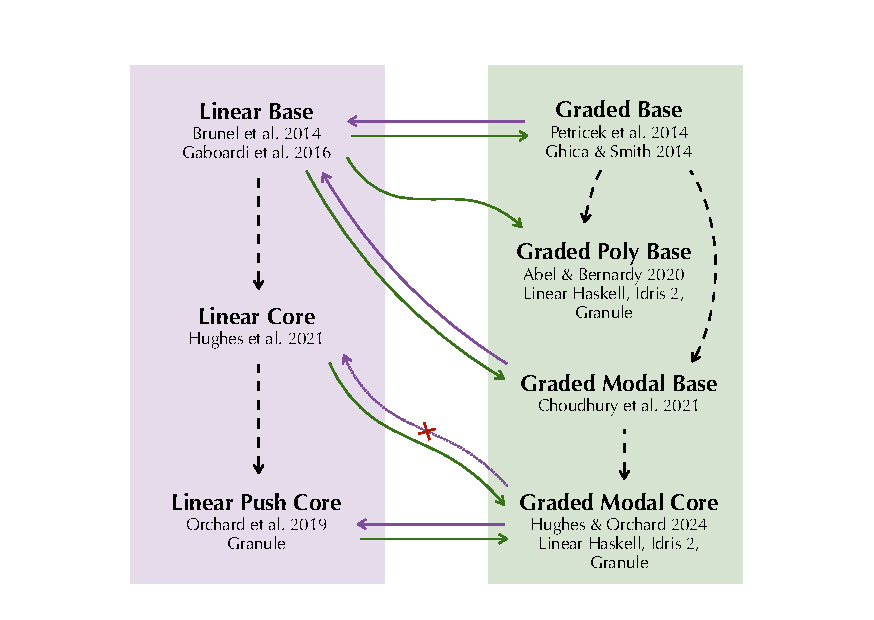
\includegraphics[width=0.6\textwidth]{linear-calculi-diagram.pdf}
	\caption{Relationship between graded calculi studied in this paper. For each calculus, a
   selection of representative papers and programming systems is given (that typically also extend the
   given calculus with orthogonal features, such as dependent types, which are not relevant to this paper). A dashed arrow denotes a
   subset relationship. A solid arrow denotes a semantics-preserving translation which we
   define in the present paper. A crossed-out arrow with a dotted shaft refers to a translation that
   is not possible.}
	\label{fig:relationship}
\end{figure}

\paragraph{Contributions and roadmap}

Our aim is to elucidate the connection between the two distinct strands of
coeffect reasoning that have emerged in the literature and in programming language
implementations, which we call \emph{linear-base} vs. \emph{graded-base} systems.
We show that, depending on the substrate, both systems can be given mutual translations to each other in a sound way.

Figure~\ref{fig:relationship}
gives an overview of these two strands, instantiated as several concrete calculi with differing
features which we summarise here with relevant section numbers:

Linear-base systems are shown on the left. Here \textbf{Linear~Base} (\ref{sec:linear-base}) represents a linear
$\lambda$-calculus extended with graded modal necessity $ \textcolor{coeffectColor}{\square_{ \SYSTEMnt{r} } }  \SYSTEMnt{A} $, corresponding to a
generalised \textit{of course} modality. \textbf{Linear~Core} (\ref{sec:linear-core}) augments this with products and sums
(multiplicative conjunction and additive disjunction). \textbf{Linear Push Core} (\ref{sec:linear-push-core}) further adds constructs for
allowing distributivity of graded modalities over products and sums, thereby losing the
correspondence to Linear Logic, as shown by \citet{hughes2021linear}. This system can model the
interaction between grades and products/sums in Granule as presented by
\citet{DBLP:journals/pacmpl/OrchardLE19}.

On the right then we have graded-base systems, for all of which \textbf{Graded~Base} (\ref{sec:graded-base}) is the
underlying calculus, corresponding to pervasively-graded simply-typed $\lambda$-calculus in the
style of \citet{petricek2014coeffects}, \citet{ghica2014bounded}, and Linear Haskell as presented by
\citet{DBLP:journals/pacmpl/BernardyBNJS18}. \textbf{Graded~Poly~Base} (\ref{sec:graded-poly-base}) augments this with
System-F-style type abstraction as in the work of \citet{DBLP:journals/pacmpl/AbelB20}, presenting a
substrate modelling more closely the actual implementation of Linear Haskell, as well as Idris 2
(where the dependent types have no interaction with grades)~\cite{DBLP:conf/ecoop/Brady21} and also
Granule with the \granin{GradedBase} language extension~\cite{DBLP:conf/esop/HughesO24}.
\textbf{Graded~Modal~Base} (\ref{sec:graded-modal-base}) instead augments Graded Base by adding a graded modal necessity akin to the
one in Linear Base. \textbf{Graded~Modal~Core} (\ref{sec:graded-core}) augments the latter system with products and sums and
thereby captures the interaction between grades and algebraic datatypes available e.g. in Granule with the
\granin{GradedBase} extension, and Linear Haskell and Idris 2 (where a modal operator can be
encoded via an algebraic datatype).

The paper is then structured as follows:

\begin{itemize}
\item
Section~\ref{sec:calculi} introduces Linear Base and Graded Base. Section \ref{sec:transl}
introduces syntax for translation, gives a \textbf{translation from Graded Base to Linear Base}
(\ref{subsec:transl-graded-base-to-linear-base}) with soundness results, and then
the converse \textbf{from Linear Base to Graded Base} via a CPS-like translation
(\ref{subsec:lin-to-grad-cps}).

\item Section~\ref{sec:calculi-with-modality} extends Graded Base to Graded Modal Base
(\ref{sec:graded-modal-base}), gives a \textbf{translation from Linear Base to Graded Modal Base}
(\ref{subsec:transl-lb2gmb}) with soundness results, gives a \textbf{translation from Graded Modal
Base to Linear Base} (\ref{subsec:transl-gmb2lb}) with soundness results, investigates the nature of
the relationship between both translations (\ref{subsec:mutual-relationship}), and gives a possible
generalisation of elimination for the graded modality that appears in the literature, along with tradeoffs
(\ref{sec:flattening}).

\item
Section~\ref{sec:poly} gives an alternative strategy for adding a graded modality to Graded Base,
via an encoding inspired by Linear Haskell, extends Graded Base to Graded Poly Base
(\ref{sec:graded-poly-base}), and gives a \textbf{translation from Linear Base to Graded Poly Base}
(\ref{subsec:transl-gpb2lb}) with soundness results.

\item
Section~\ref{sec:prods-sums} adds product and sum types, allowing us to study the interaction of
coeffects with data structures. It extends Linear Base to Linear Core (\ref{sec:linear-core}), extends
Graded Modal Base to Graded Modal Core (\ref{sec:graded-core}), gives a \textbf{translation from
Linear Core to Graded Modal Core} (\ref{sec:linear-core-to-graded}) with soundness results, shows
\textbf{there is no sound translation from Graded Modal Core to Linear Core}
(\ref{sec:no-trans-graded-core-to-linear-core}), extends Linear Core to Linear Push Core
(\ref{sec:linear-push-core}), and gives a \textbf{translation from Graded Modal
Core to Linear Push Core} with soundness results.

\item
Section~\ref{sec:discussion} asks: \textit{is one approach better than the other?}
(\ref{sec:better}), gives some simple example programs in languages that implement features from the
two lineages studied (\ref{sec:wild}, considers some related ideas (\ref{sec:comparison-with-effects}-\ref{sec:raos}), and concludes (\ref{sec:conclusion}).
\end{itemize}
%
